\section{Reconstruction and Samples from the DukeMTMC Dataset}
\label{app:duke_visual}

\begin{center}
    \begin{minipage}[c]{0.49\linewidth}
        \centering
        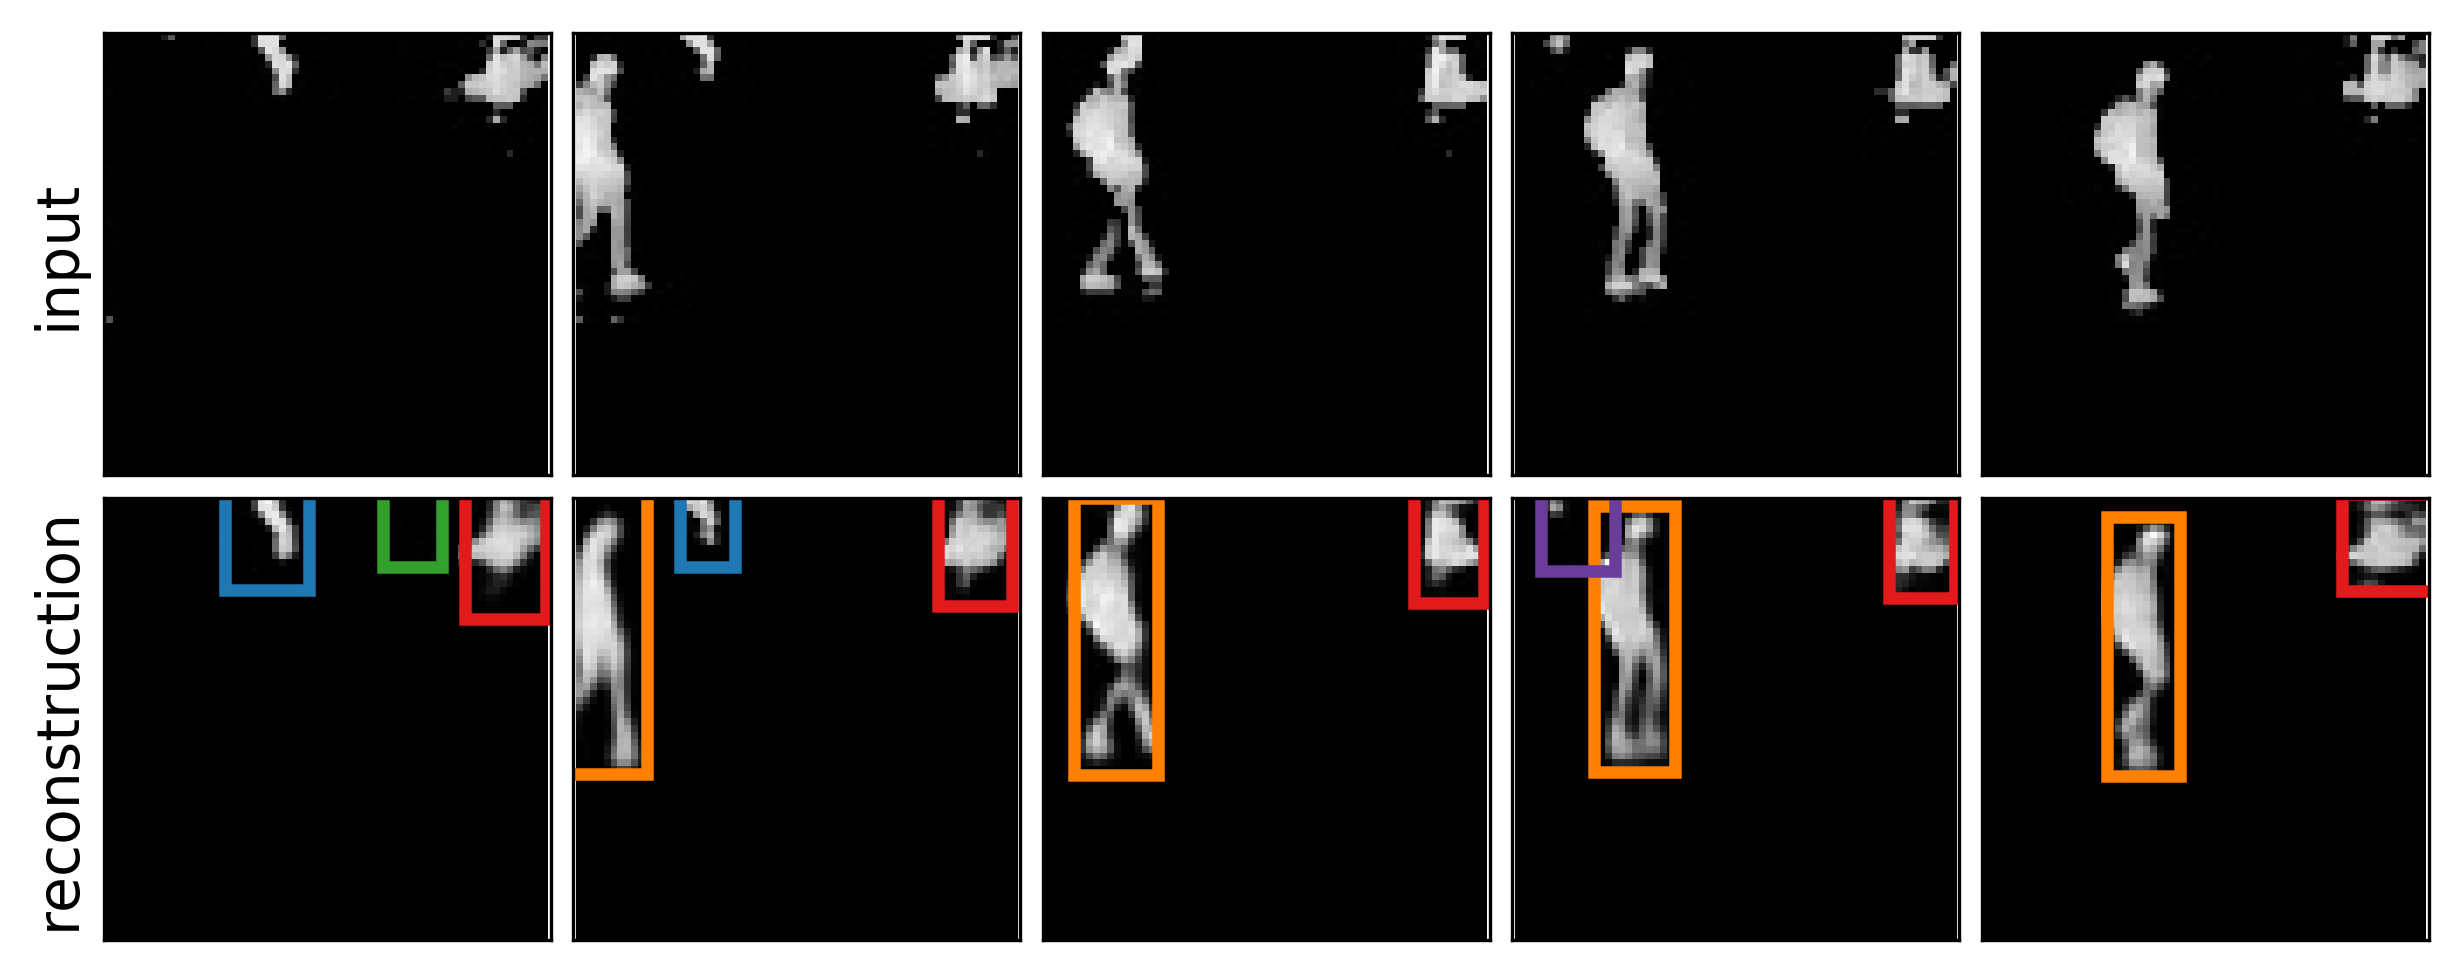
\includegraphics[width=\linewidth]{figures/SQAIR/duke_rec/000093.png}
        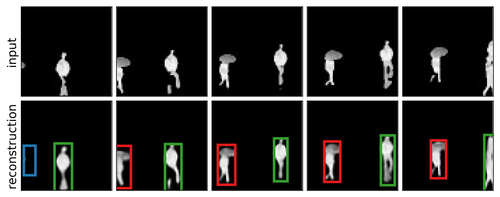
\includegraphics[width=\linewidth]{figures/SQAIR/duke_rec/000045.png}
        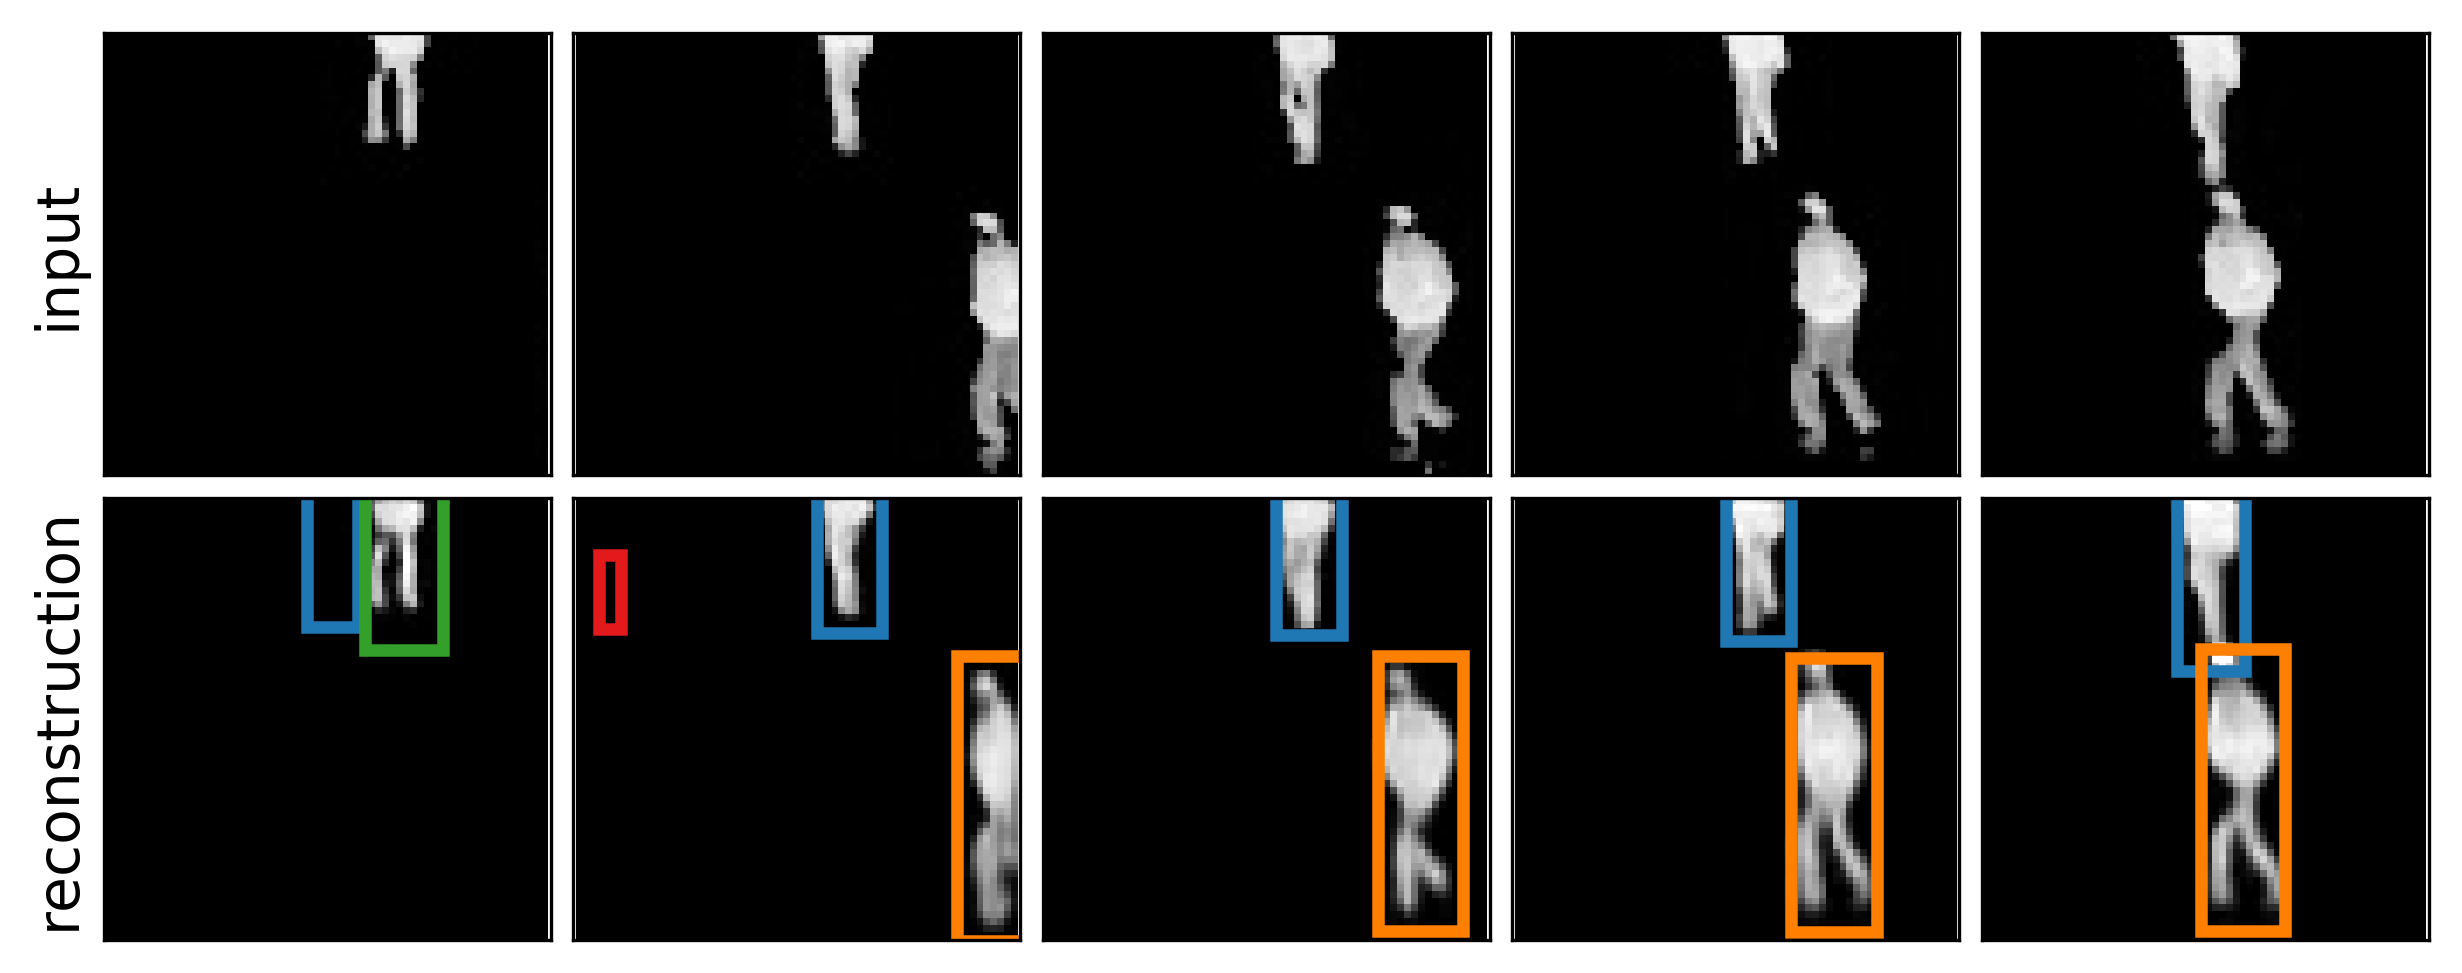
\includegraphics[width=\linewidth]{figures/SQAIR/duke_rec/000047.png}
        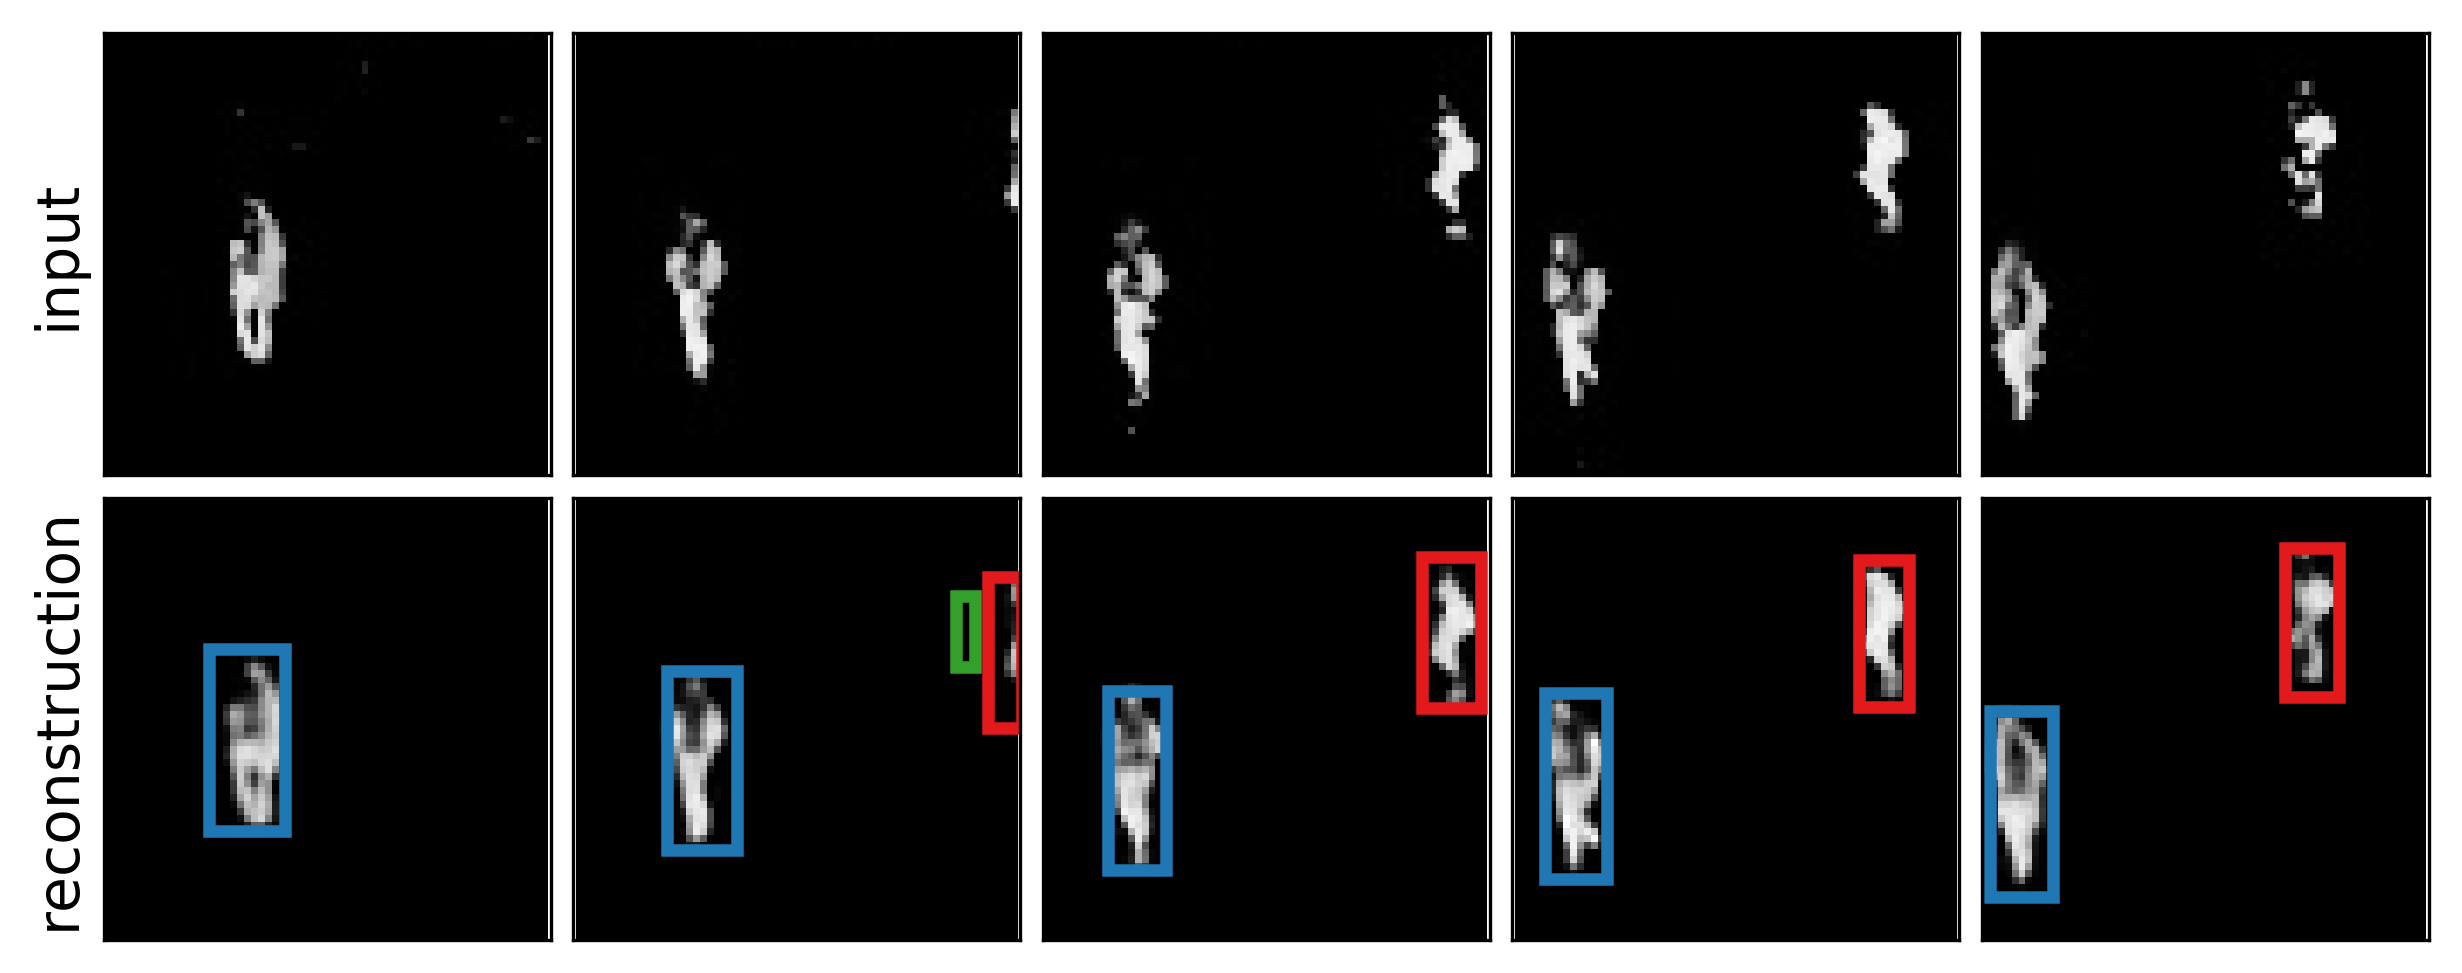
\includegraphics[width=\linewidth]{figures/SQAIR/duke_rec/000081.png}
        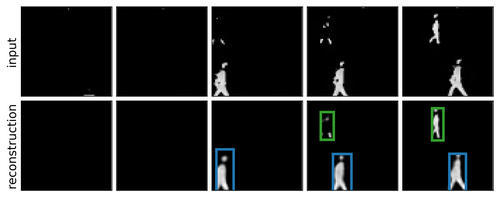
\includegraphics[width=\linewidth]{figures/SQAIR/duke_rec/000085.png}
    \end{minipage}
    \hfill
    \begin{minipage}[c]{0.49\linewidth}
        \centering
        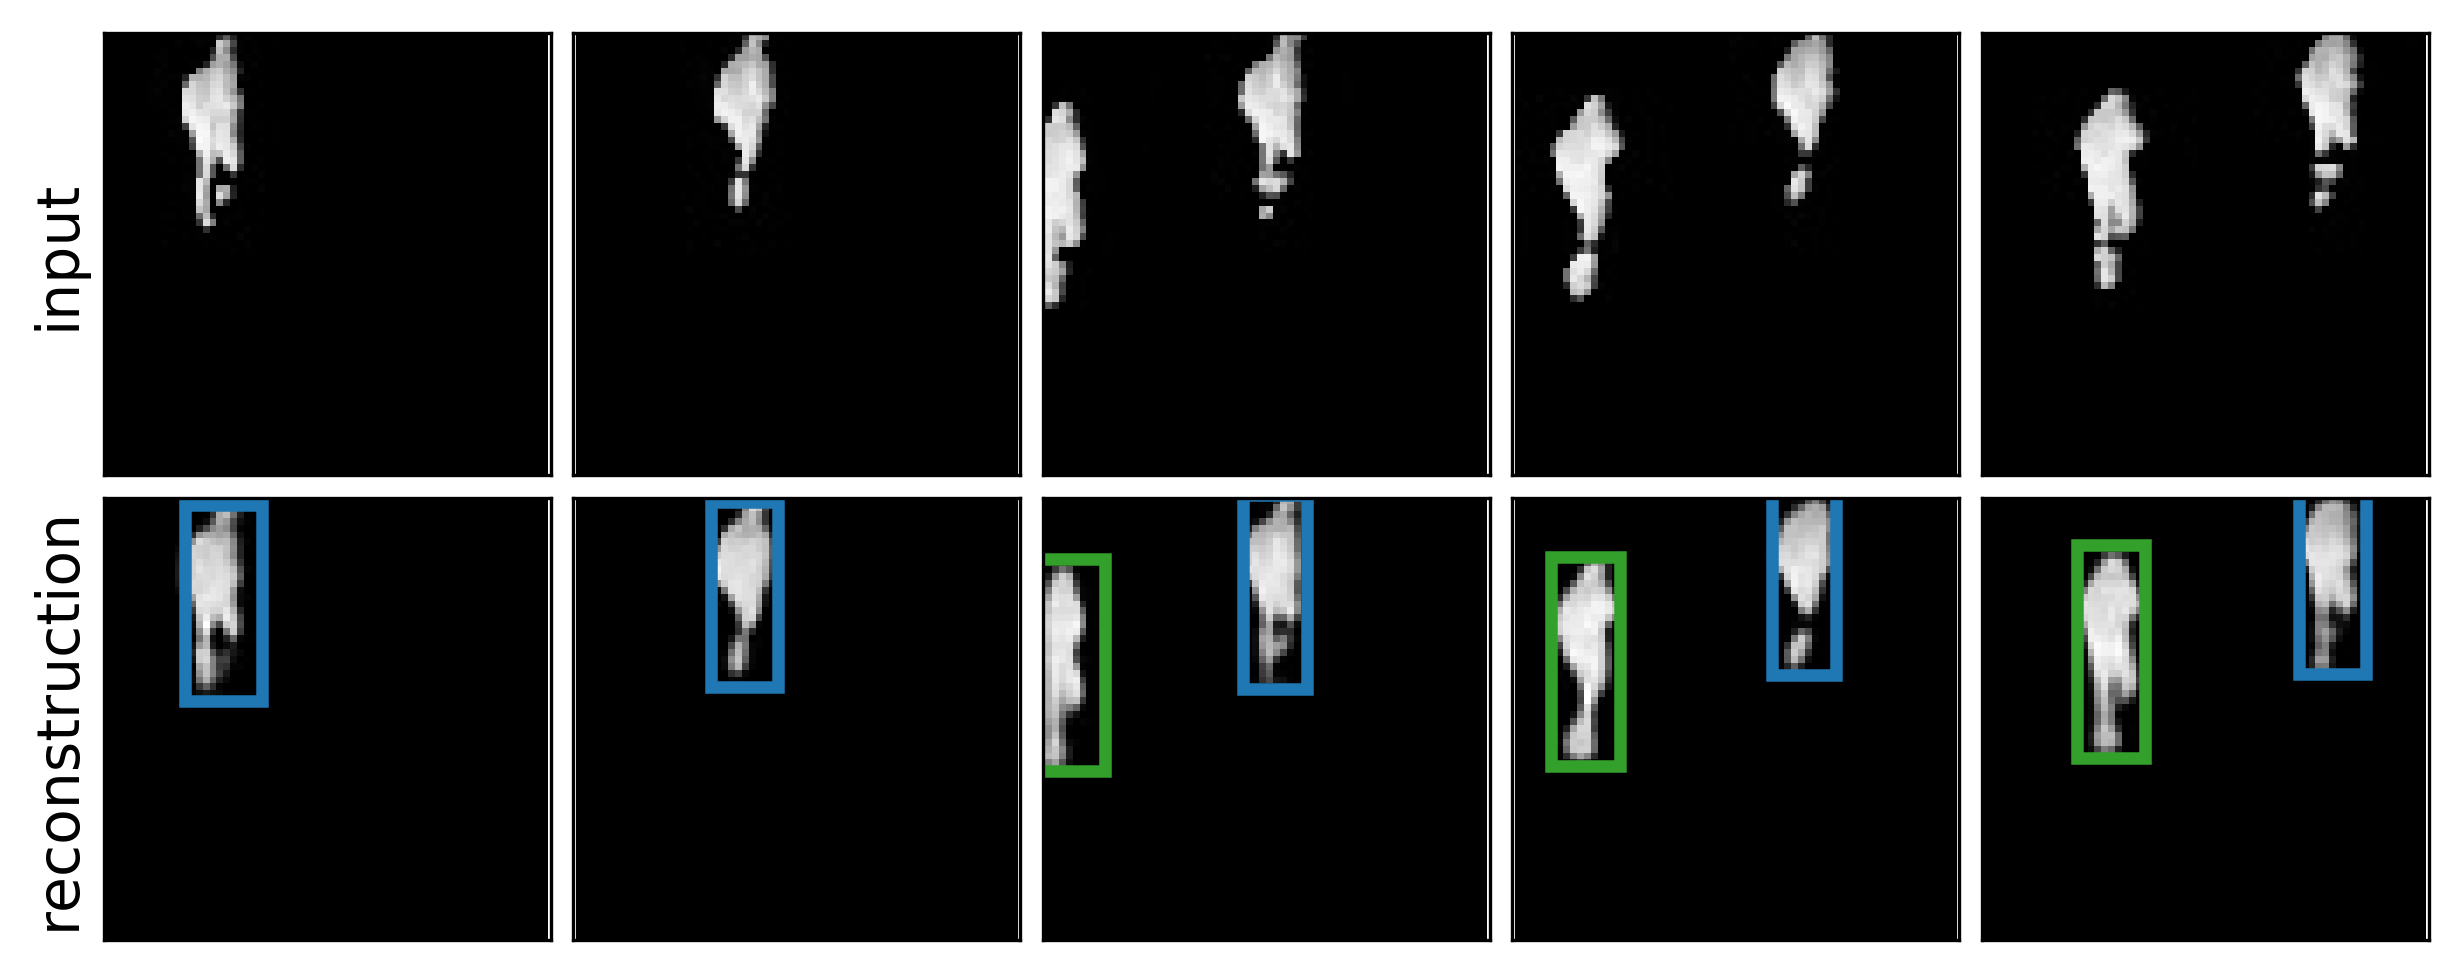
\includegraphics[width=\linewidth]{figures/SQAIR/duke_rec/000088.png}
        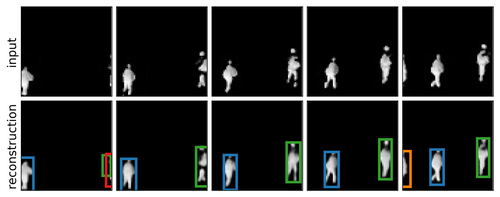
\includegraphics[width=\linewidth]{figures/SQAIR/duke_rec/000046.png}
        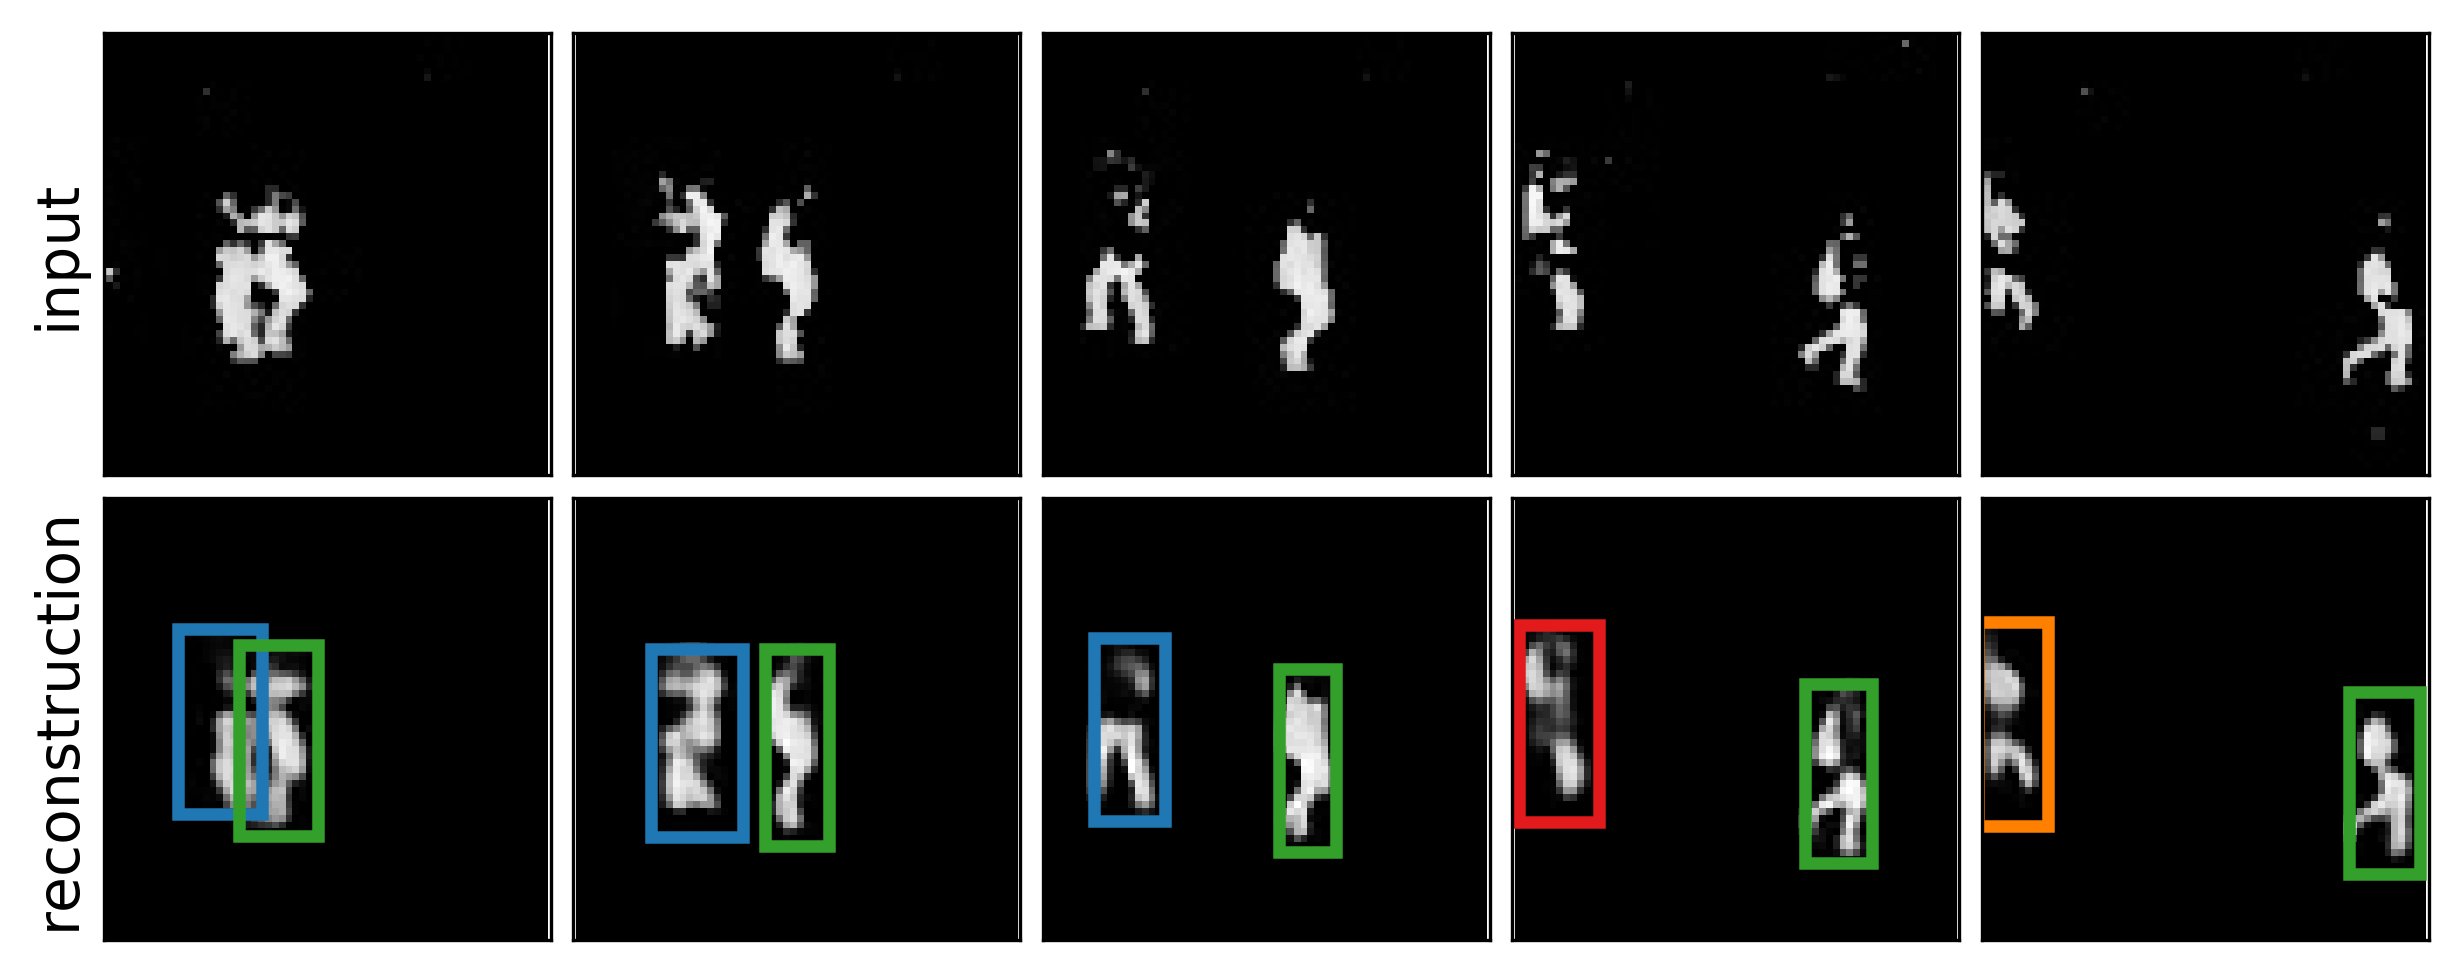
\includegraphics[width=\linewidth]{figures/SQAIR/duke_rec/000094.png}
        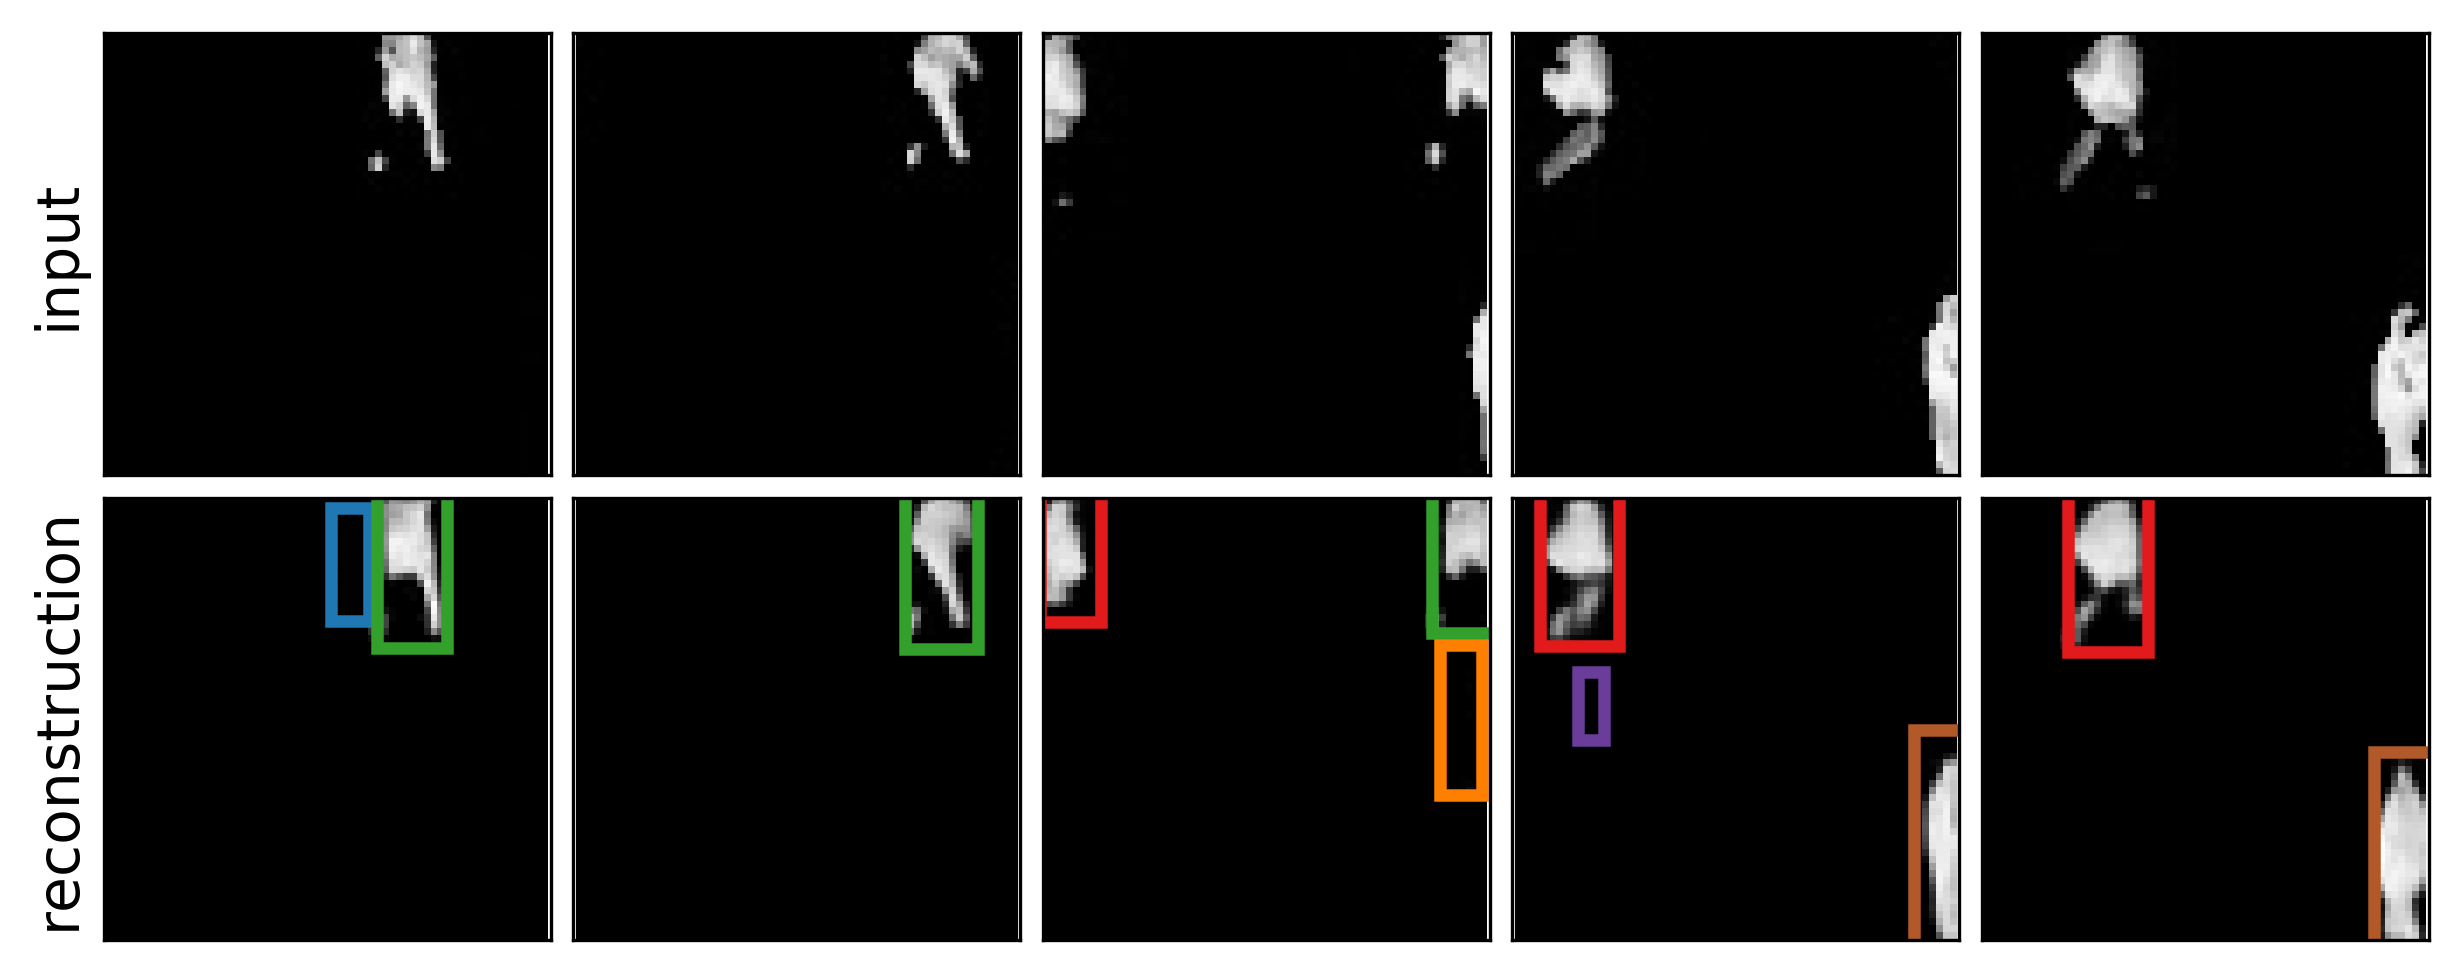
\includegraphics[width=\linewidth]{figures/SQAIR/duke_rec/000096.png}
        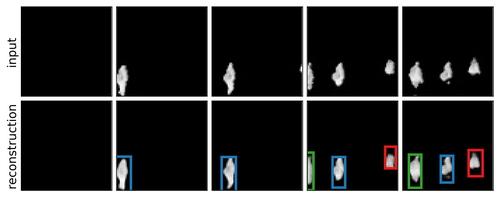
\includegraphics[width=\linewidth]{figures/SQAIR/duke_rec/000108.png}
    \end{minipage}
    \captionof{figure}{Sequences of input (first row) and \gls{SQAIR} reconstructions with marked glimpse locations. While not perfect (spurious detections, missed objects), they are temporally consistent and similar in appearance to the inputs.}
    \label{fig:duke_recs_additional}
\end{center}

\begin{center}
    \begin{minipage}[c]{0.49\linewidth}
        \centering
         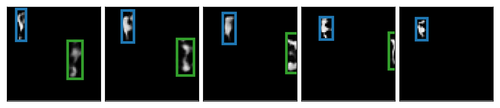
\includegraphics[width=\linewidth]{figures/SQAIR/duke_sample/000078.png}
        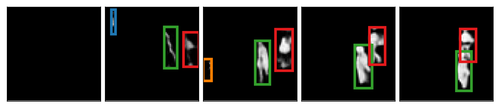
\includegraphics[width=\linewidth]{figures/SQAIR/duke_sample/000250.png}
        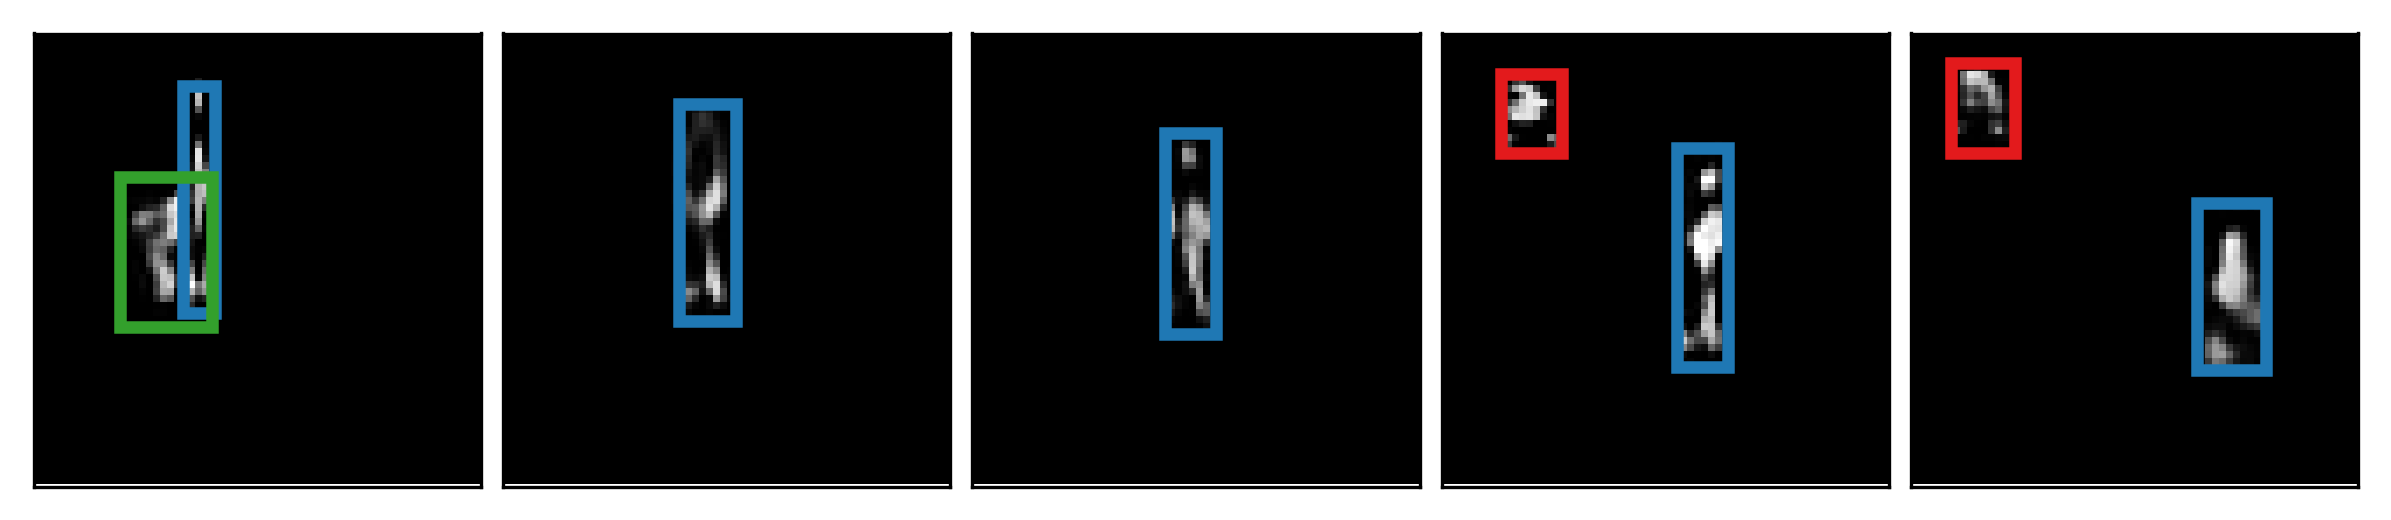
\includegraphics[width=\linewidth]{figures/SQAIR/duke_sample/000005.png}
        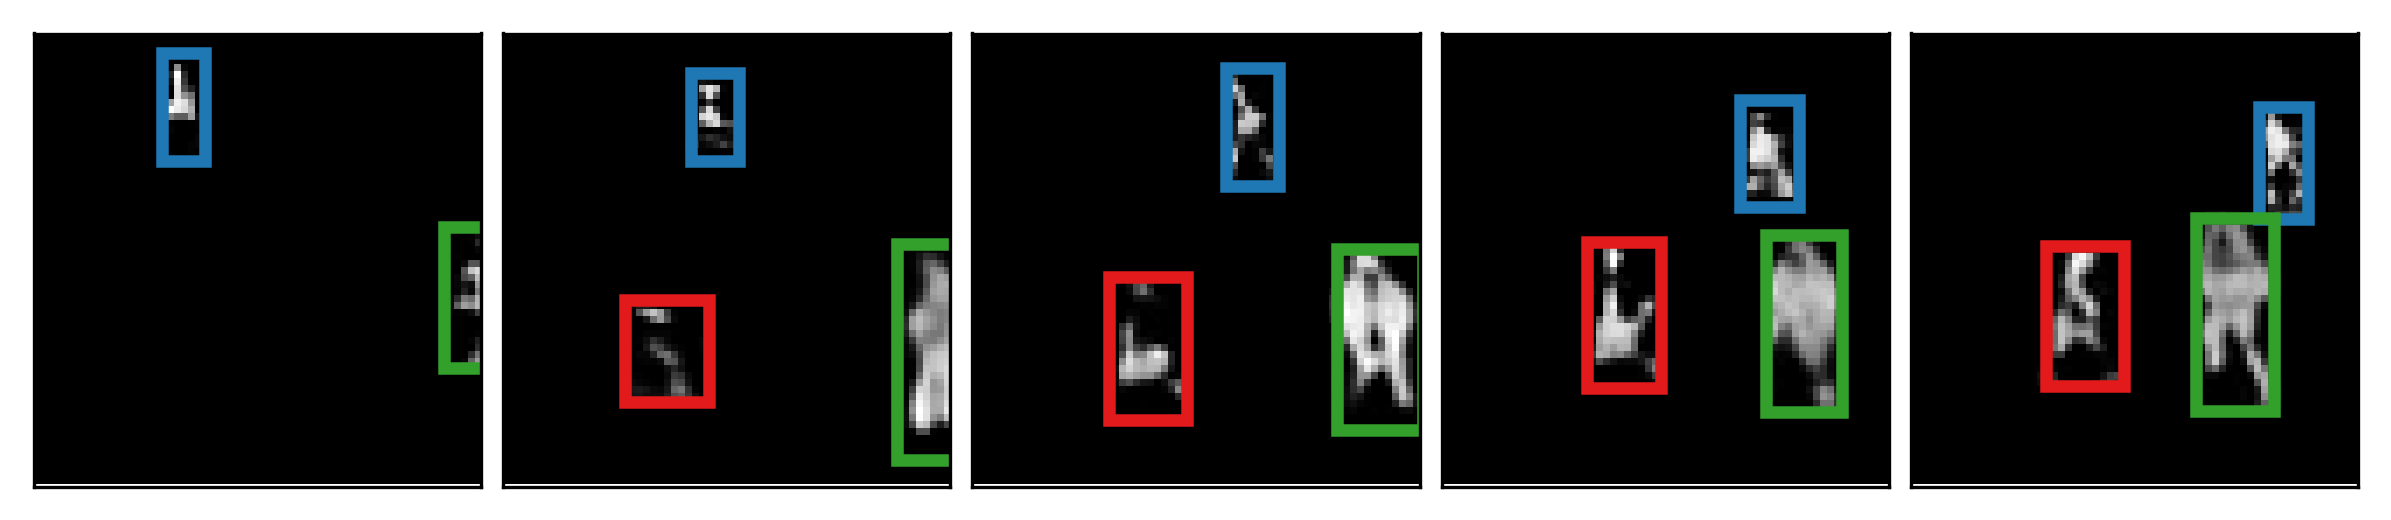
\includegraphics[width=\linewidth]{figures/SQAIR/duke_sample/000015.png}
        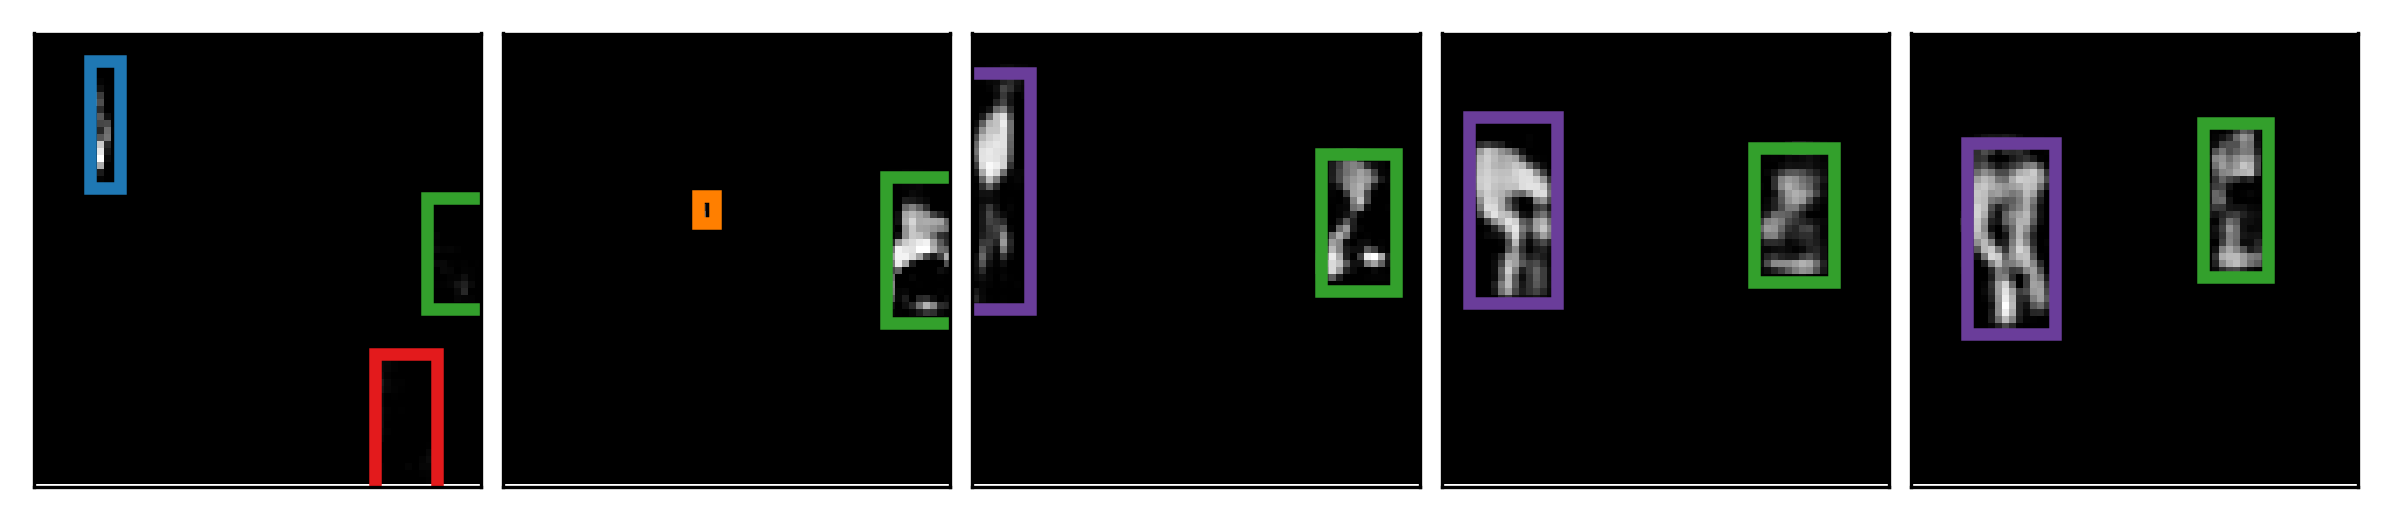
\includegraphics[width=\linewidth]{figures/SQAIR/duke_sample/000019.png}
        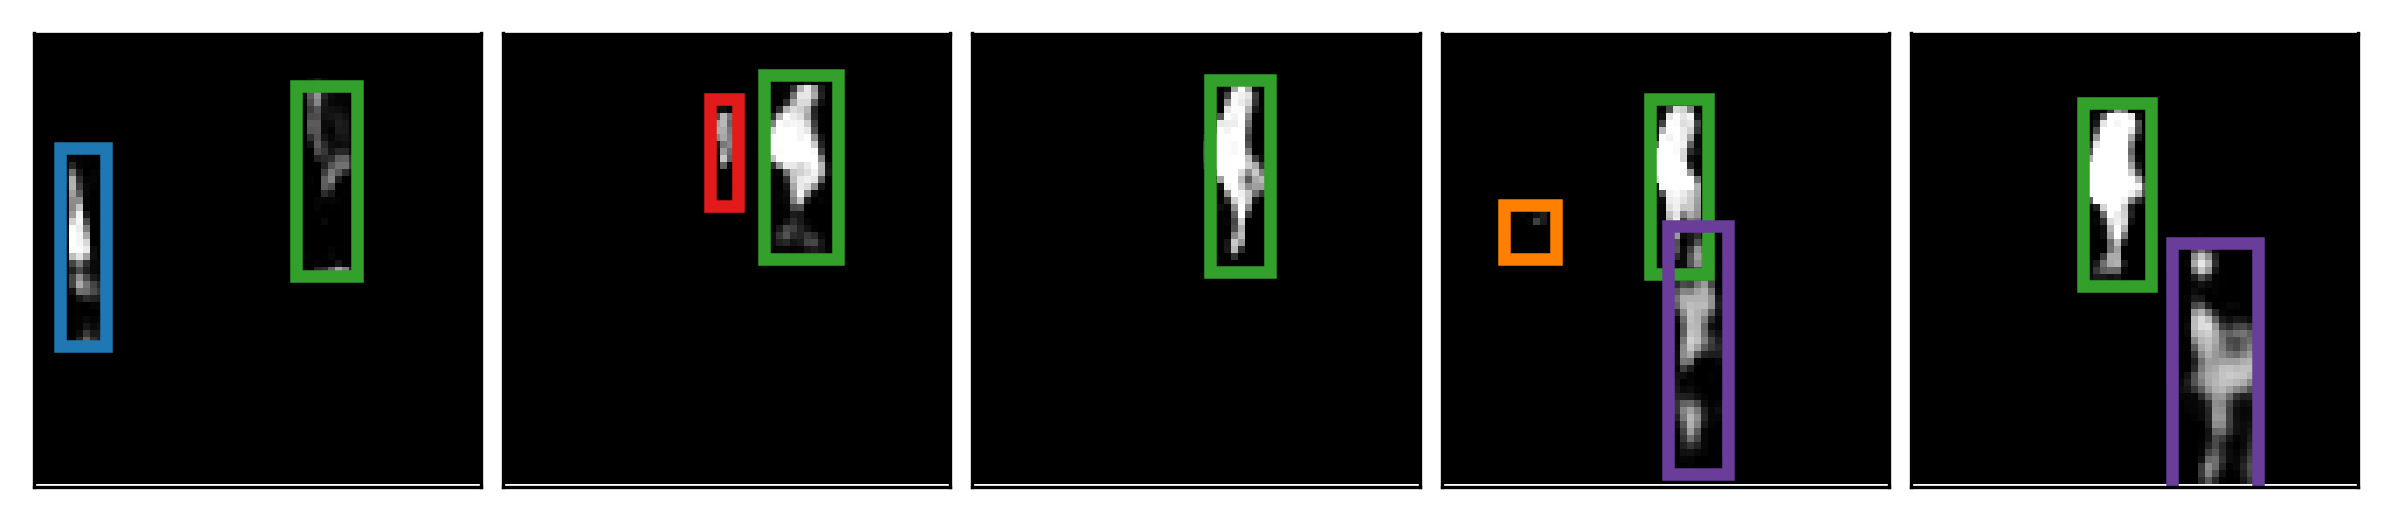
\includegraphics[width=\linewidth]{figures/SQAIR/duke_sample/000023.png}
        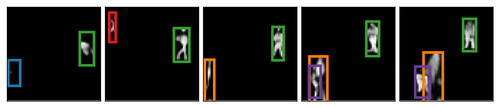
\includegraphics[width=\linewidth]{figures/SQAIR/duke_sample/000038.png}
        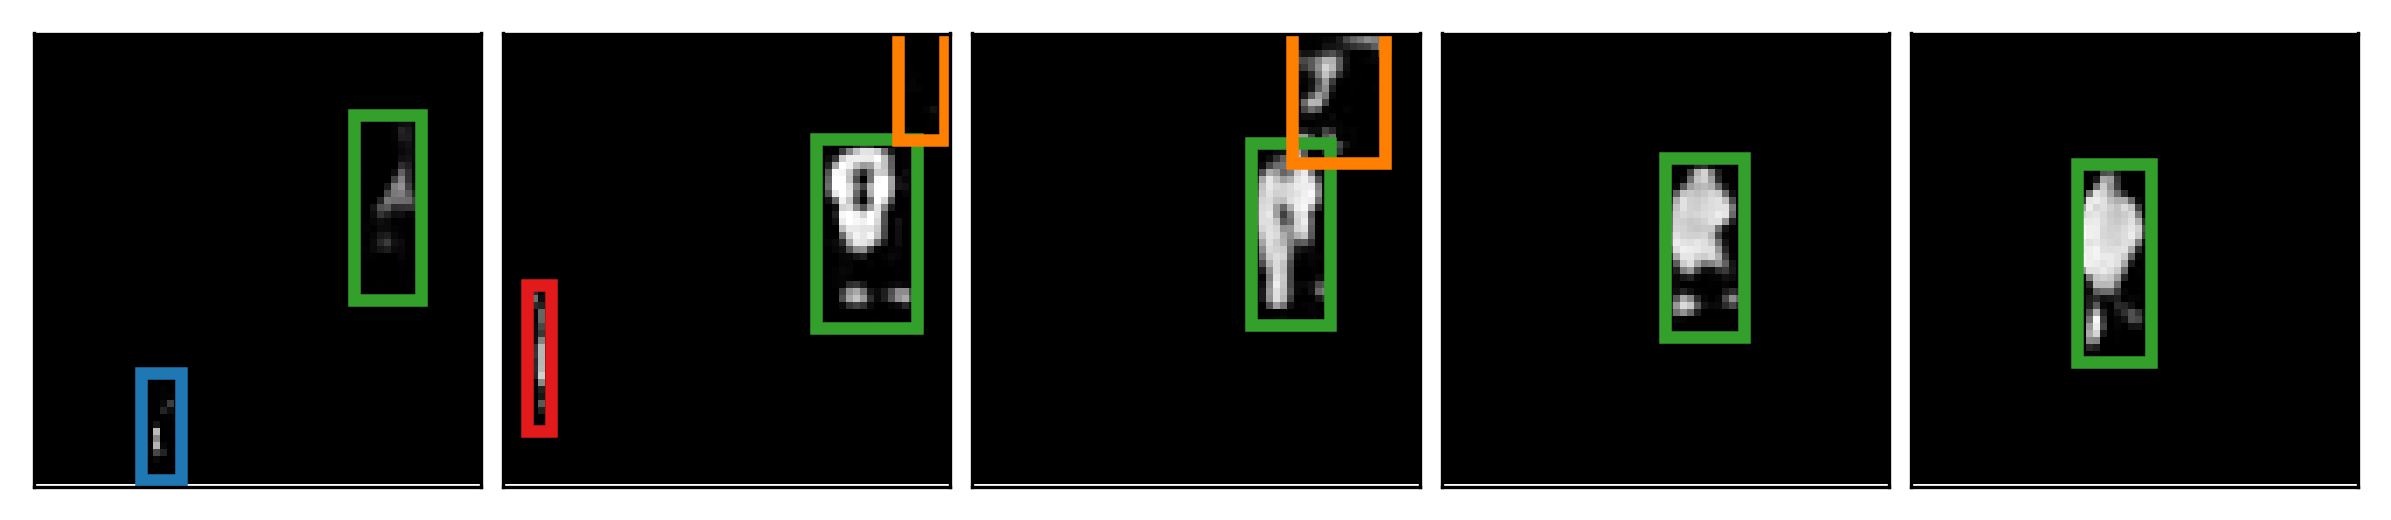
\includegraphics[width=\linewidth]{figures/SQAIR/duke_sample/000062.png}
    \end{minipage}
    \hfill
    \begin{minipage}[c]{0.49\linewidth}
        \centering
            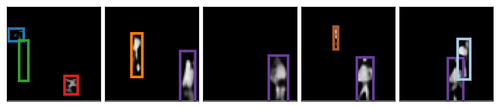
\includegraphics[width=\linewidth]{figures/SQAIR/duke_sample/000225.png}
        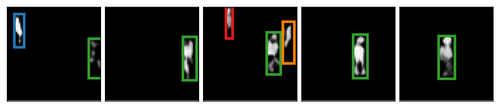
\includegraphics[width=\linewidth]{figures/SQAIR/duke_sample/000121.png}
        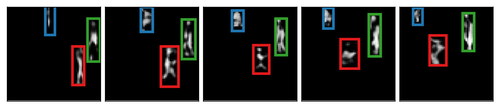
\includegraphics[width=\linewidth]{figures/SQAIR/duke_sample/000128.png}
        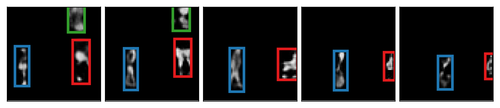
\includegraphics[width=\linewidth]{figures/SQAIR/duke_sample/000132.png}
        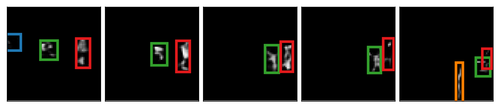
\includegraphics[width=\linewidth]{figures/SQAIR/duke_sample/000134.png}
        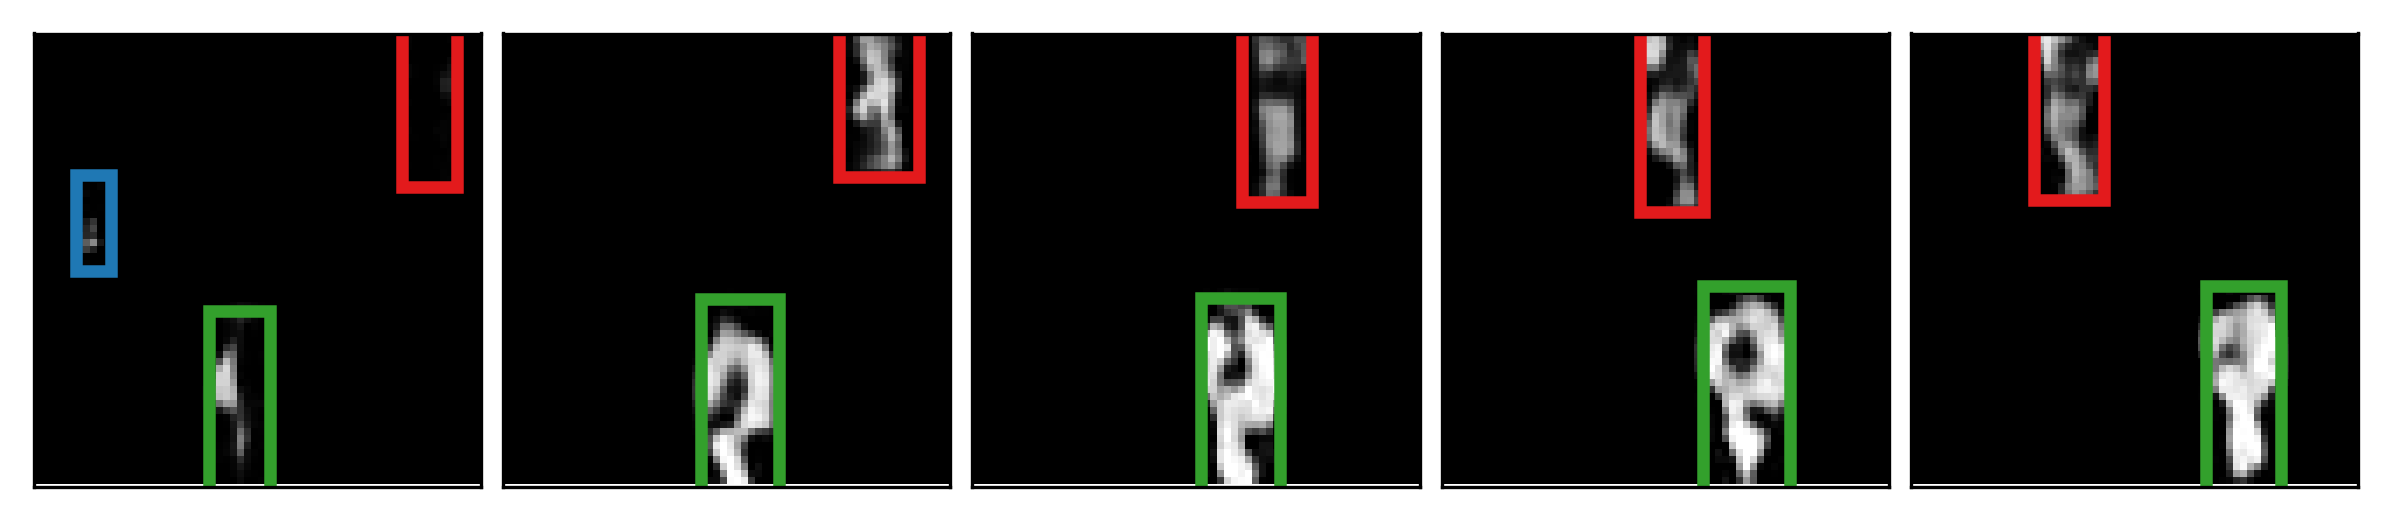
\includegraphics[width=\linewidth]{figures/SQAIR/duke_sample/000140.png}
        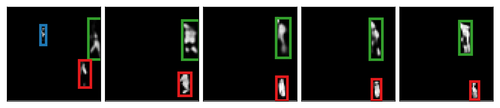
\includegraphics[width=\linewidth]{figures/SQAIR/duke_sample/000144.png}
    \end{minipage}
    \captionof{figure}{Samples with marked glimpse locations from \gls{SQAIR} trained on the DukeMTMC dataset. Both appearance and motion is spatially consistent. Generated objects are similar in appearance to pedestrians in the training data. Samples are noisy, but so is the dataset.}
    \label{fig:duke_samples_additional}
\end{center}

\begin{center}
    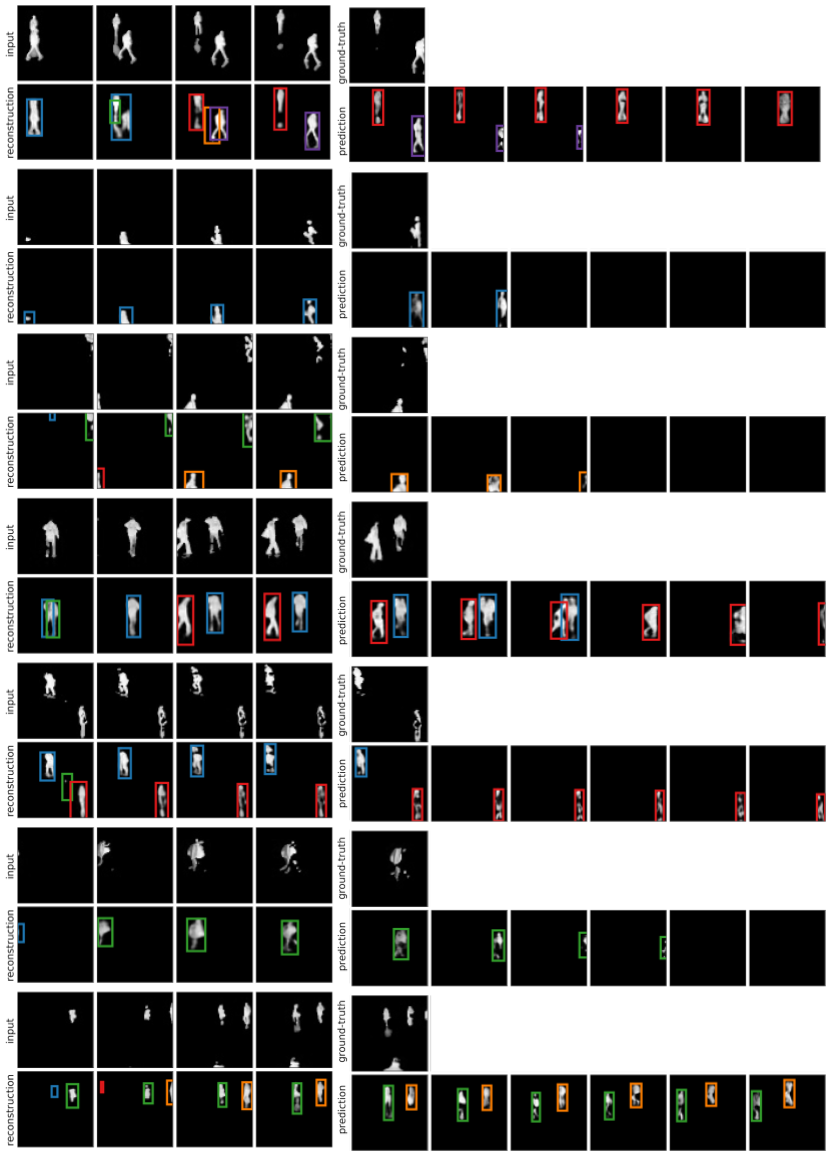
\includegraphics[width=\linewidth]{figures/SQAIR/duke_cond_gen/sqair_duke_cond_gen_appendix.png}
    \captionof{figure}{Conditional generation from \gls{SQAIR}, which sees only the first four frames in every case. Top is the input sequence (and the remaining ground-truth), while bottom is reconstruction (first four time-steps) and then generation.}
    \label{fig:duke_cond_gen_sqair}
\end{center}